\section{Suggested Defense Mechanisms}
\label{sec:defense}

In this section, we suggest a few defense mechanisms to mitigate the proposed attacks. Particularly, to defend against the remote attacks, we propose an OAuth-based protocol to prevent unauthorized apps from exploiting the standard SDK and TGSP, and a signature-based mechanism to counter the malicious SDK and malicious TGSP server; to defend against the proximate attack, we propose to employ a strong encryption algorithm such as AES to eliminate possible eavesdropping attacks. Note that since all these defense methods are patching-based solutions that require the efforts from the manufacture (NeuroSky), we are not able to implement them; but they can %We are hoping that the defense discussion of this section can 
serve as security suggestions to most health-related IoT manufactures for the purpose of enhancing the security of their products. We also discuss the possible side-channel attacks that could occur even if the data are well protected by adopting certain defense mechanisms. Such a discussion signals that securing health-based IoT systems has a long-way to go, and this endeavor deserves a lot more effort from both academia and industry.

\subsection{Solutions to Mitigate Remote Attacks}

\subsubsection{OAuth-Based Framework}

The root cause of the EEG data leak to malicious applications through SDK and TGSP is because the EEG system framework lacks necessary authentication/authorization. Noticing this deficiency,  we propose to apply OAuth~\cite{hardt2012oauth}, a well-known authorization and authentication protocol, in the EEG system framework for eliminating the attacks resulted from unauthorized malicious applications. Since the traditional OAuth protocol was designed for three-party authorization, while the EEG system framework involves four parties, we modify the OAuth protocol to fit into the EEG system framework and present the details in the following paragraph.

We demonstrate in Figure~\ref{fig:oauth} how the OAuth 2.0 implicit granting protocol can be applied in the EEG system framework. This OAuth-patched EEG framework requires NeuroSky to maintain a service-providing server on which all BCI-app developers have to register their newly developed BCI apps before these apps can be downloaded by the users. When a BCI-app developer registers a new BCI app with the service-providing server, the BCI app is assigned with an app ID and an app secret (normally a random hash given by the service-providing server). When the BCI app wishes to access a user's EEG data through TGSP or SDK, the following process needs to be performed: (1) the BCI app passes its app ID and app secret %to the TGSP server or \texttt{thinkgear.dll}; (2) the TGSP server or \texttt{thinkgear.dll} forwards the app ID and app secret 
to the NeuroSky service-providing server; (2) the user is directed to the NeuroSky service-providing server and is notified of the requesting app ID; (3) the service-providing server first checks if the requesting app ID and app secret match with that the developer registered; if not, the request is denied directly; otherwise, the user is asked by the service-providing server whether or not he wishes to grant the permission to the app to access his EEG data; (4) if granted, the service-providing server passes an access token back simultaneously to the BCI app and to the TGSP server or the \texttt{thinkgear.dll}; %(5) the TGSP server or the \texttt{thinkgear.dll} forwards the token to the BCI app; 
(5) the BCI app authenticates itself with the TGSP server or \texttt{thinkgear.dll} using the access token; and (6) the BCI app obtains the EEG data if passes the access token verification. 
Note that even though this modified OAuth protocol has four parties involved, it operates in the same way as the original one. As one can see, after thinkgear.dll or TGSP server gets a copy of the access token, it immediately becomes a new service-providing server and continues the OAuth. Therefore, our modified OAuth protocol preserves the same security strength as the original one. 


\begin{figure}[!htb]
\hspace*{2cm}
        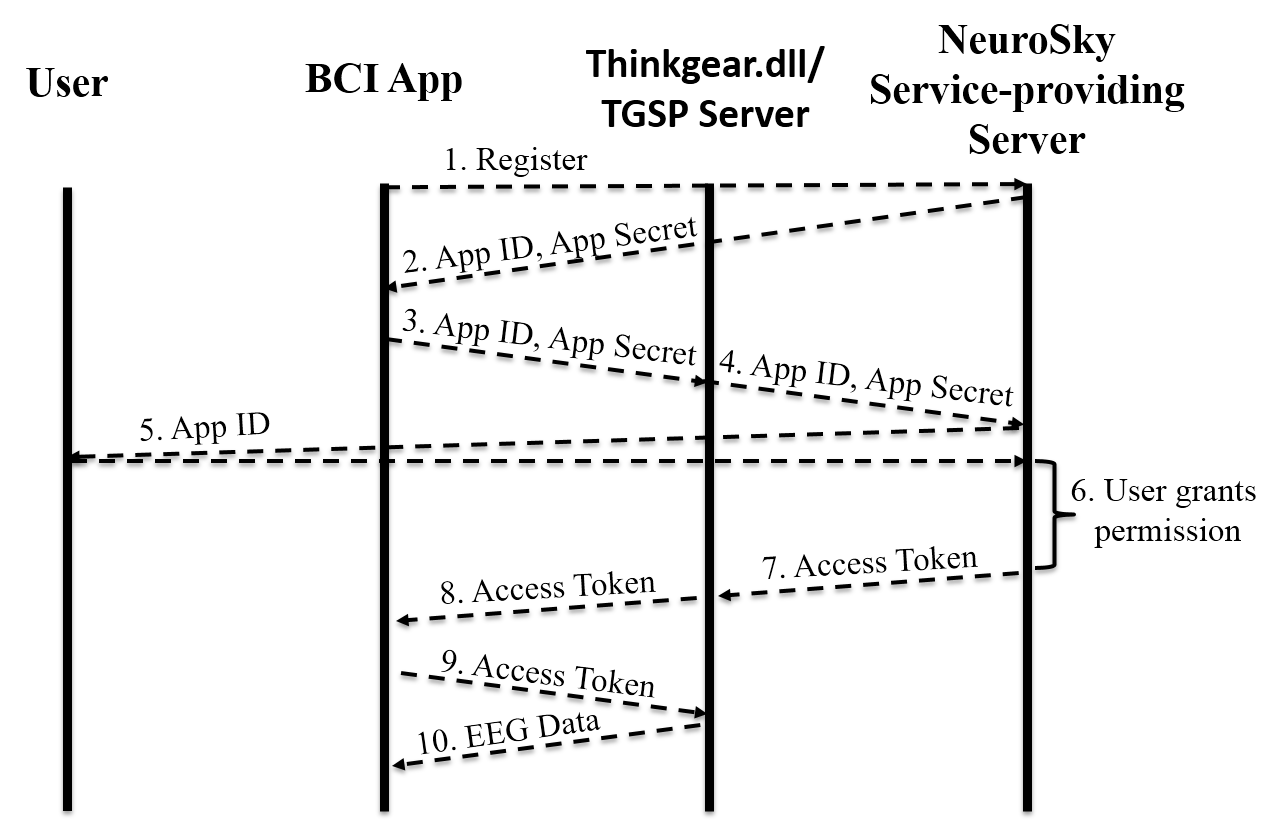
\includegraphics[scale=0.3]{oauth.png}
	\caption{The OAuth 2.0 implicit granting protocol applied to EEG system framework. }
        \label{fig:oauth}
\end{figure}

Also note that to adopt the OAuth protocol, we need to enforce secure communications among the entities. In other words, the communications between a BCI app and the NeuroSky service-providing server, between thinkgear.dll/TGSP server and the NeuroSky service-providing server, and between a BCI app and thinkgear.dll/TGSP server, must be secured since their transmissions contain sensitive information such as the app secret and access token. We suggest that the communications between a BCI app and the NeuroSky service-providing server and between thinkgear.dll/TGSP server and the NeuroSky service-providing server directly adopt the SSL/TLS protocol for traffic encryption since they are using TCP for message transmissions. As for the communications between a BCI app and thinkgear.dll/TGSP server, if they reside on the same PC, one can directly employ the OS-level inter-process communications (IPC) which automatically secure the transmissions due to the sandbox feature; if they are not on the same PC, one can adopt the SSL/TLS protocol. On the other hand, even though the communications between a user and the NeuroSky service-providing server do not contain sensitive information, however, if without traffic encryption, an attacker can tamper the app ID so that the user can mistakenly grant permissions to an unauthorized app; thus the SSL/TLS protocol is also suggested to secure the message transmissions. 

\subsubsection{Signature-Based Solution}
NeuroSky does not implement any tamper-resistant technique, thus allowing an attacker to arbitrarily modify or fabricate its binary programs such as \texttt{thinkgear.dll} and the TGSP server, as we have done to construct our malicious TGSP server and SDK in Subsections~\ref{sec:malicious:TGSP} and \ref{sec:malicious:SDK}. An intuitive defense mechanism to counter such attacks is to employ software verification via digital signatures. An app then can verify the signature of the SKD or the TGSP server before interacting with them for EEG data acquisition. As a malicious SDK or TGSP server also reads data from the RF dongle, the dongle should be able to verify their authenticity; this requires NeuroSky to re-implement the firmware on the dongle as the current version is not able to perform signature verification. 

%Digital signature is a widely-adopted mechanism for protecting applications from unauthorized modifications. It is consisted with two parts, generation and verification. In the generation step, NeuroSky first needs to generate a hash for each of the protected programs, i.e, \texttt{thinkgear.dll} and TGSP server. Then NeuroSky leverages one the asymmetric encryption algorithms by first generating a pair of public key and private key, then using the private key to encrypt the hashes, and finally inserting the encrypted hashes and the digital signature (the public key and the plaintext hashes), into the protected programs. In the verification step, before interacting with \texttt{thinkgear.dll} or the TGSP server, every BCI app should first extract the published digital signature and use the public key to decrypt the encrypted hashes, and compare whether the decrypted hashes are matched with the original plaintext hashes. If they are matched, it means the protected programs are intact, otherwise, it means that protected programs have been modified and the BCI apps should terminate the interactions. Digital signature is mature and widely-adopted in the industry, many off-the-shelf tools provide generation and verification services. SignTool is one of the most commonly-used tools developed by Microsoft for this purpose~\cite{signtool}.

\subsection{Solution to Mitigate the Proximate Attack}

Our proximate attack proposed in Subsection~\ref{sec:proximate:attack} actually is a type of eavesdropping attack that requires signal recording and replaying in order to recover the original EEG data. To mitigate this attack, a well-examined encryption algorithm such as AES is suggested. This requires the NeuroSky headset and the RF dongle to pre-share a secret key or employ a practical key management protocol for key generation to secure their communications. Obviously, such a defense mechanism requires firmware upgrade in the RF dongle.

%In order to inhibit the proximate attack, one could eliminate the possibility of replay attack. Simple encryption methods for radio frequency such as voice inversion, hopping inversion and rolling code inversion are easy to be cracked and are vulnerable to replay attacks. However, the computation power of the EEG devices limits the use of some complex encryption protocols, e.g., secure sockets layer (SSL). Having realized this, we suggest adopting advanced encryption standard (AES) for secure EEG data transmission. \textcolor{blue}{In order to do so, the NeuroSky headset uses a secret key as a secret key to encrypt the EEG data using AES, then the RF dongle decrypt the encrypted data with the secret key using AES to obtain the raw EEG data. The key problem is the key distribution and management. Adopting  Diffie-Hellman key exchange protocol~\cite{diffie1976new}, agreeing on a pre-shared key, or maintaining a trusted sever and adopting attribute-based encryption~\cite{bethencourt2007ciphertext} are a new options. By adopting the solution properly, NeuroSky can effectively inhibit the proximate attack.}


\subsection{Discussions on Possible Side-Channel Leaks}
Even if the EEG data are properly protected based on our proposed defense mechanisms, inference attacks exploiting side-channel information may be difficult to avoid. In this subsection, we discuss the possible side-channel-based inference attacks a remote attacker and a proximate attacker can launch. As mentioned earlier, it is impossible for us to implement the suggested defense mechanisms in the NeuroSky EEG framework; thus it is impossible for us to construct the proposed side-channel attacks. 

\subsubsection{Remote Side-Channel Attacks}
In a remote side-channel attack, the attacker has a malicious program running on the victim's PC. If adopting the OAuth protocol and the digital signature protection methods, the malicious program is unable to conduct any remote attacks mentioned in Section~\ref{sec:attack}. However, it can still capture the USB traffic coming in and out of the RF dongle using a popular USB protocol~\cite{usbprotocol}. Nevertheless, the packet structure of the USB protocol is somehow highly similar to the ones in the network protocols such as TCP and UDP. As demonstrated by Saltaformaggio \emph{et al.} in \cite{brendan2016}, fine-grained user activities can be inferred from the encrypted network traffic. Therefore it is highly possible for an attacker to recover a user's brain status by monitoring the USB traffic coming in and out of the RF dongle.

\subsubsection{Proximate Side-Channel Attacks}
In a proximate attack, the attacker does not have access to the victim's PC but is within certain range of the victim. By encrypting the radio signals between the NeuroSky headset and the RF dongle, the attacker is not able to conduct the record-and-replay based eavesdropping attack presented in section~\ref{sec:proximate:attack} to recover the victim's EEG data. However, the attacker can still record the encrypted radio wave, which is a kind of electromagnetic wave. As demonstrated by Song \emph{et al.}~\cite{song2016my}, an attacker can infer what object a 3D printer prints by exploiting the electromagnetic waves. Therefore, it is highly possible for an attacker to recover a user's brain status by monitoring the encrypted radio waves emitted from the headset.
